\documentclass{beamer}

\usepackage[utf8]{inputenc}
\usepackage{hyperref}

\usetheme{Berkeley}
\beamertemplatenavigationsymbolsempty
\setbeamertemplate{headline}{}
 
\title{Creating a Workflow in FoodChain-Lab 2}
\date{}
 
\begin{document}
\maketitle

\section{Tasks}
\begin{frame}
	\begin{itemize}
		\item Use the \textbf{Tracing View} to display the delivery graph in a clearly arranged way.
		\item Apply the \textbf{Default Highlighting} to color the graph.
		\item Visualize the backward and forward trace for an arbitrary station.
	\end{itemize}
\end{frame}
 
\section{1}
\begin{frame}
	\begin{center}
  		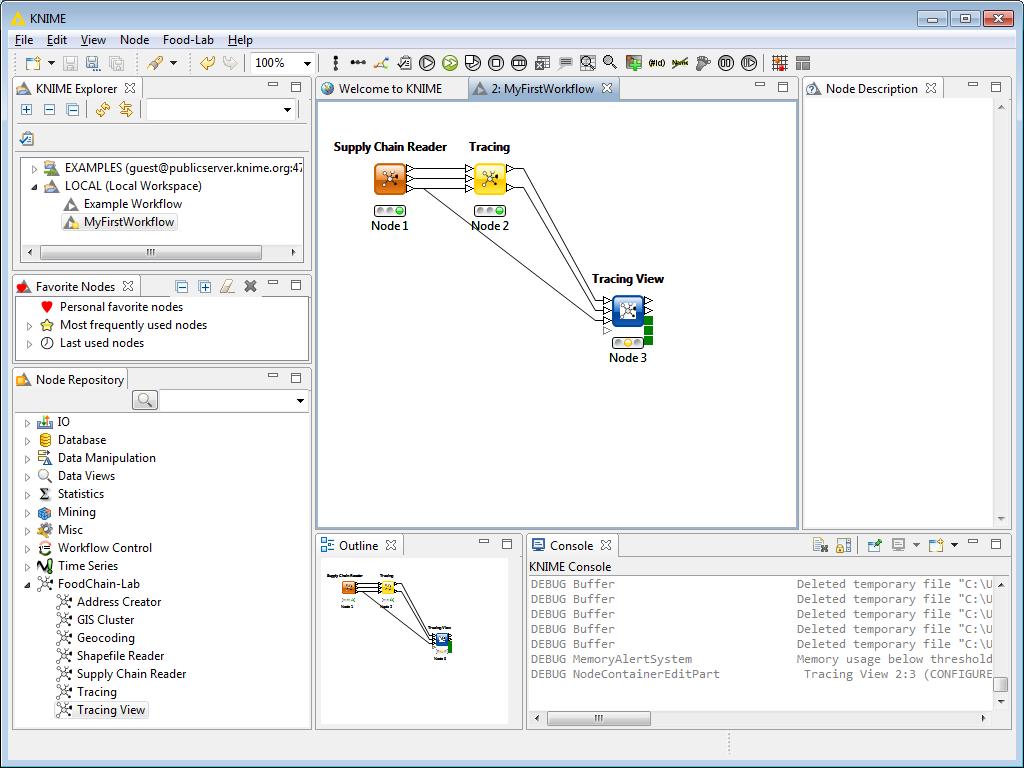
\includegraphics[height=0.6\textheight]{1.png}
	\end{center}
	\begin{itemize}
		\item This is the second part of the tutorial.
		\item You can either do the first part to create this workflow or download it from \url{https://github.com/SiLeBAT/BfROpenLabResources/raw/master/GitHubPages/workflows/MyFirstWorkflow.zip}.
		\item Double click on the \textbf{Tracing View} to open its dialog.
	\end{itemize}
\end{frame}

\section{2}
\begin{frame}
	\begin{center}
  		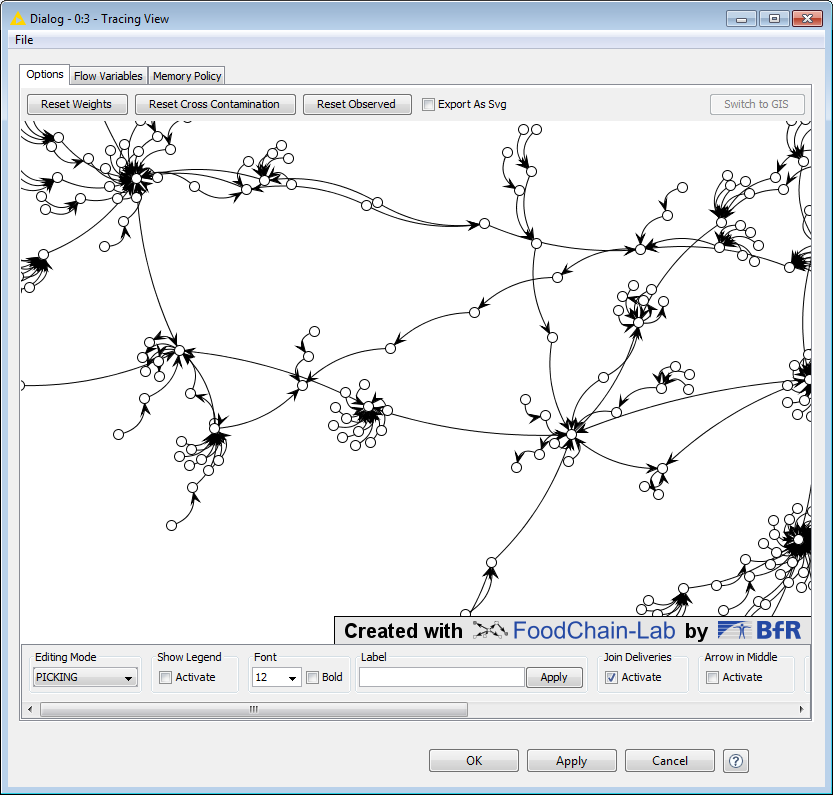
\includegraphics[height=0.6\textheight]{2.png}
	\end{center}
	\begin{itemize}
		\item In the \textbf{Tracing View} you can see the imported delivery network.
	\end{itemize}
\end{frame}

\section{3}
\begin{frame}
	\begin{center}
  		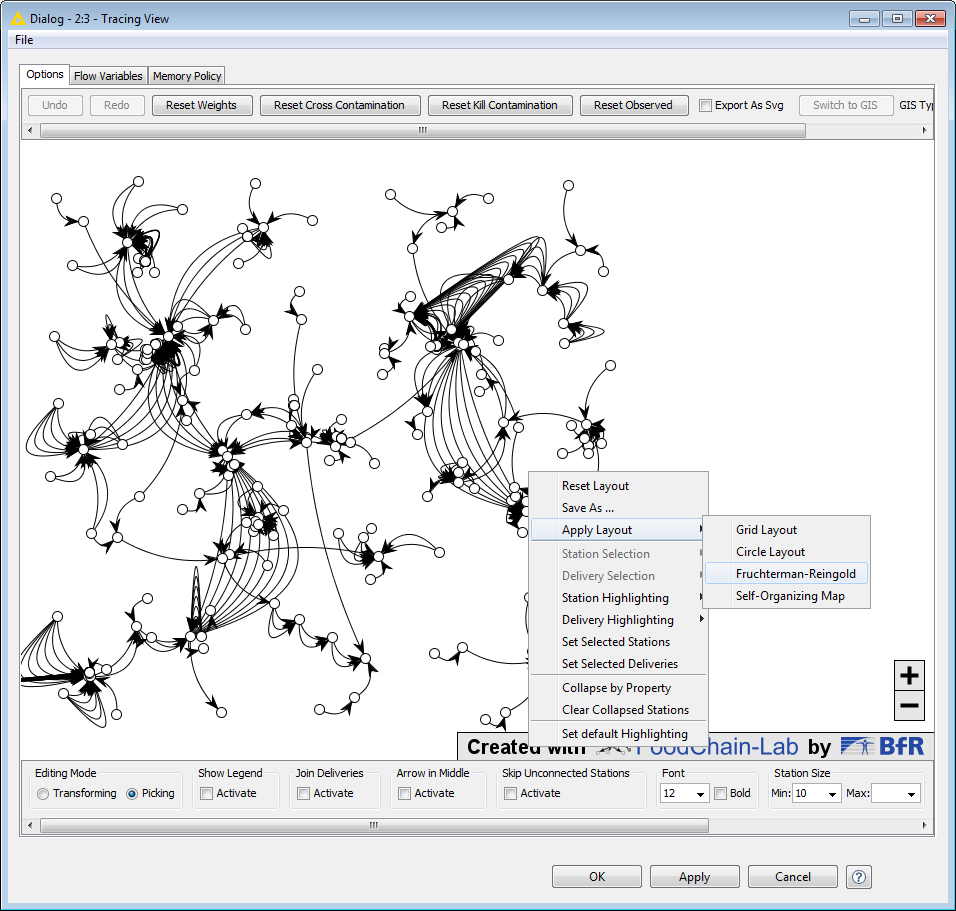
\includegraphics[height=0.6\textheight]{3.png}
	\end{center}
	\begin{itemize}
		\item To arrange the network in a better way right click in the graph and select \textbf{Apply Layout $>$ Fruchterman-Reingold}.
	\end{itemize}
\end{frame}

\section{4}
\begin{frame}
	\begin{center}
  		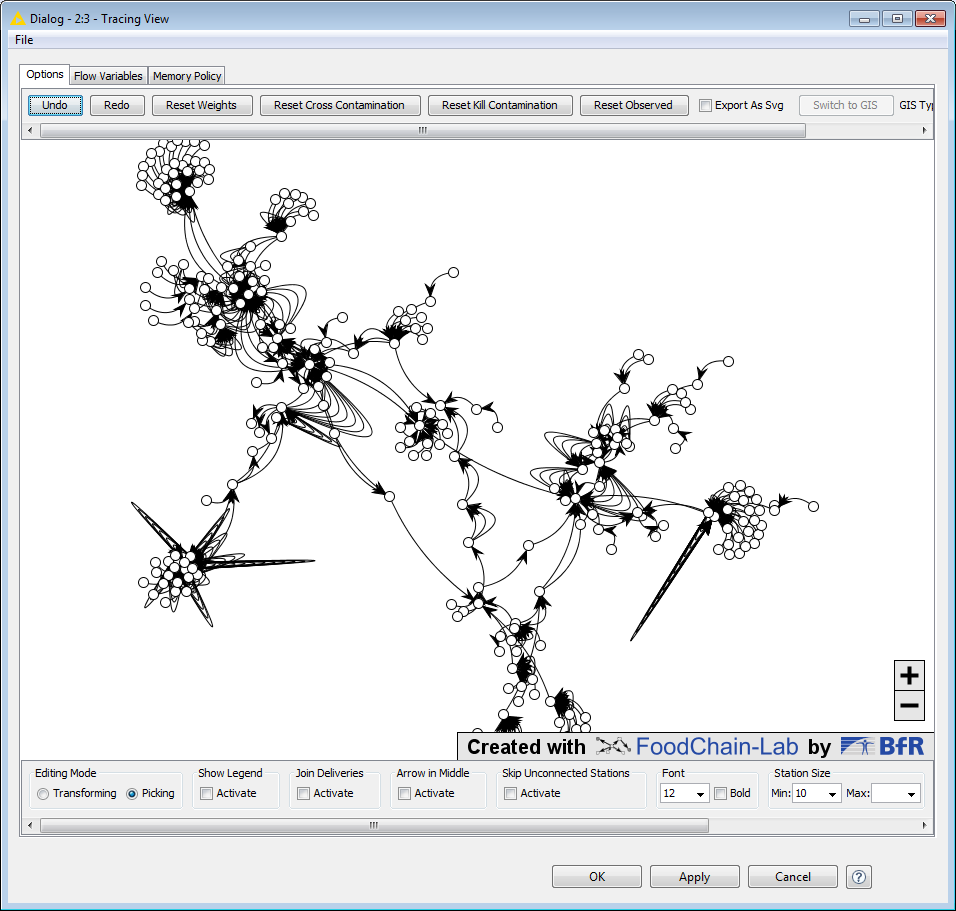
\includegraphics[height=0.6\textheight]{4.png}
	\end{center}
	\begin{itemize}
		\item This layout prozess is not deterministic. That means you will get a different result each time.
		\item You can apply the layout again, if you are not satisied with the current result.
	\end{itemize}
\end{frame}

\section{5}
\begin{frame}
	\begin{center}
  		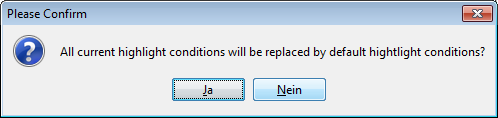
\includegraphics[height=0.6\textheight]{5.png}
	\end{center}
	\begin{itemize}
		\item Right click in the graph to open the context menu and select \textbf{Set default Highlighting}.
		\item Highlighting uses colors and sizes to visualize certain properties of stations/deliveries.
	\end{itemize}
\end{frame}

\section{6}
\begin{frame}
	\begin{center}
  		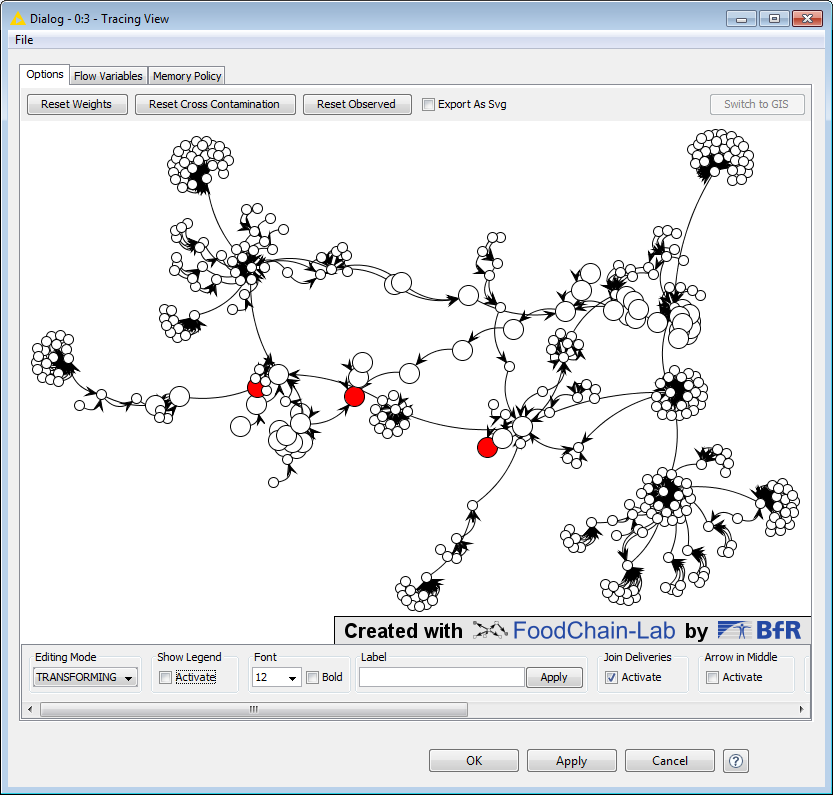
\includegraphics[height=0.6\textheight]{6.png}
	\end{center}
	\begin{itemize}
		\item You will notice, that 4 stations are colored red now and some stations increased in size.
		\item The red stations are the supermarkets, where set the weight to "1".
		\item The size of each station is based on its "Score".
	\end{itemize}
\end{frame}

\section{7}
\begin{frame}
	\begin{center}
  		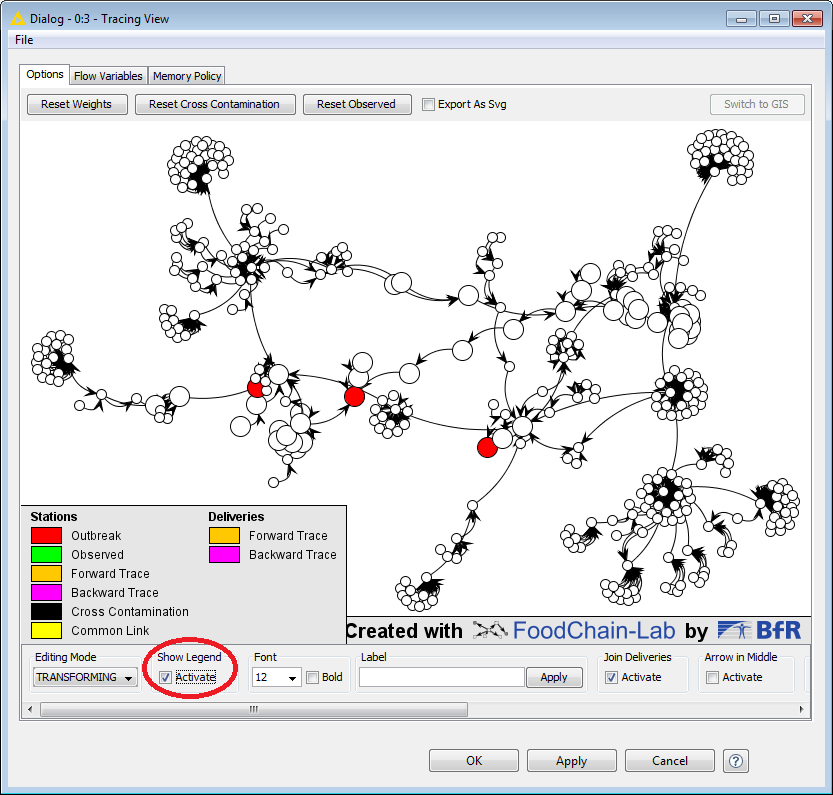
\includegraphics[height=0.6\textheight]{7.png}
	\end{center}
	\begin{itemize}
		\item Activate \textbf{Show Legend} to get a legend for the used colors.
	\end{itemize}
\end{frame}

\section{8}
\begin{frame}
	\begin{center}
  		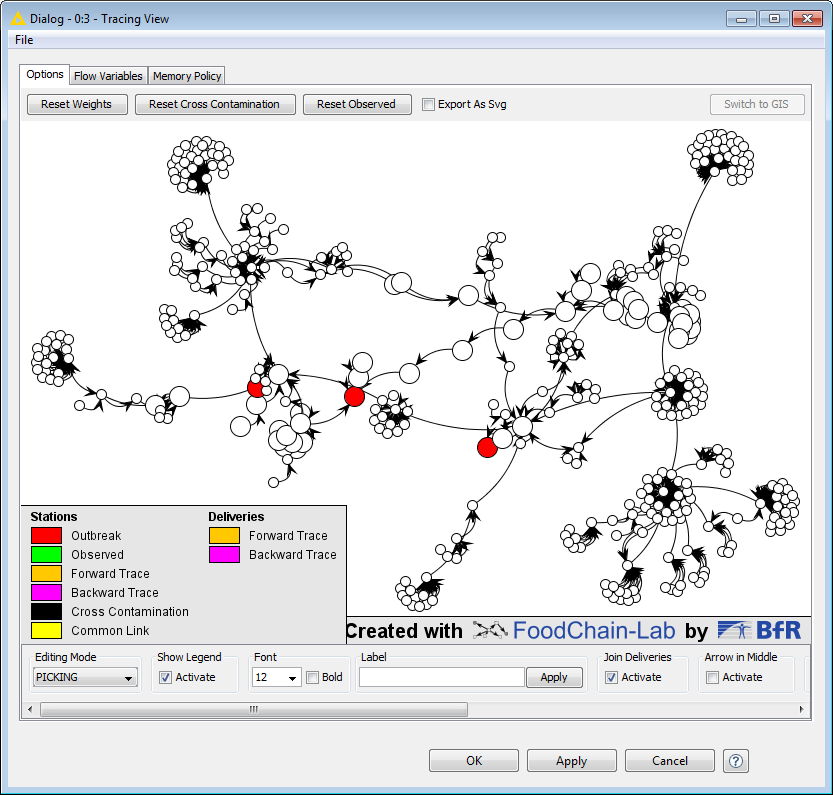
\includegraphics[height=0.6\textheight]{8.png}
	\end{center}
	\begin{itemize}
		\item Now we can observe a station to see its delivery trace.
		\item Set "Picking" as \textbf{Editing Mode} and double click on any station.
		\item We clicked on the station in the red circle.
	\end{itemize}
\end{frame}

\section{9}
\begin{frame}
	\begin{center}
  		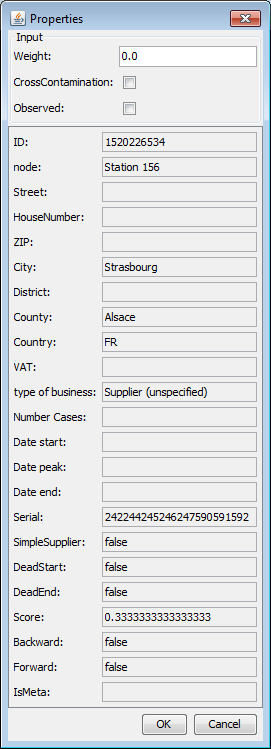
\includegraphics[height=0.6\textheight]{9.png}
	\end{center}
	\begin{itemize}
		\item A dialog will pop up, that all attributes of the station.
		\item Additionally you can change "Weight", "Cross Contamination", "Kill Contamination" and "Observed".		
	\end{itemize}
\end{frame}

\section{10}
\begin{frame}
	\begin{center}
  		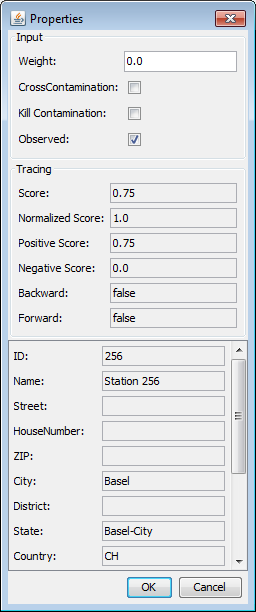
\includegraphics[height=0.6\textheight]{10.png}
	\end{center}
	\begin{itemize}
		\item Select \textbf{Observed} and press \textbf{OK}.
	\end{itemize}
\end{frame}

\section{11}
\begin{frame}
	\begin{center}
  		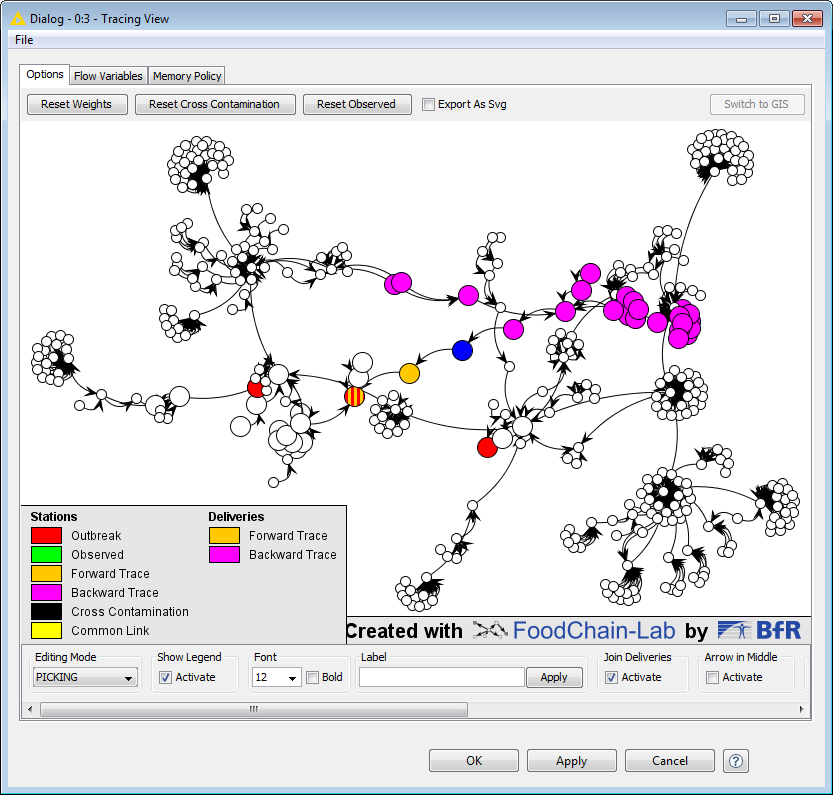
\includegraphics[height=0.6\textheight]{11.png}
	\end{center}
	\begin{itemize}
		\item All stations/deliveries of the forward trace are orange-colored and the ones of the backward trace are purple.		
	\end{itemize}
\end{frame}

\section{12}
\begin{frame}
	\begin{center}
  		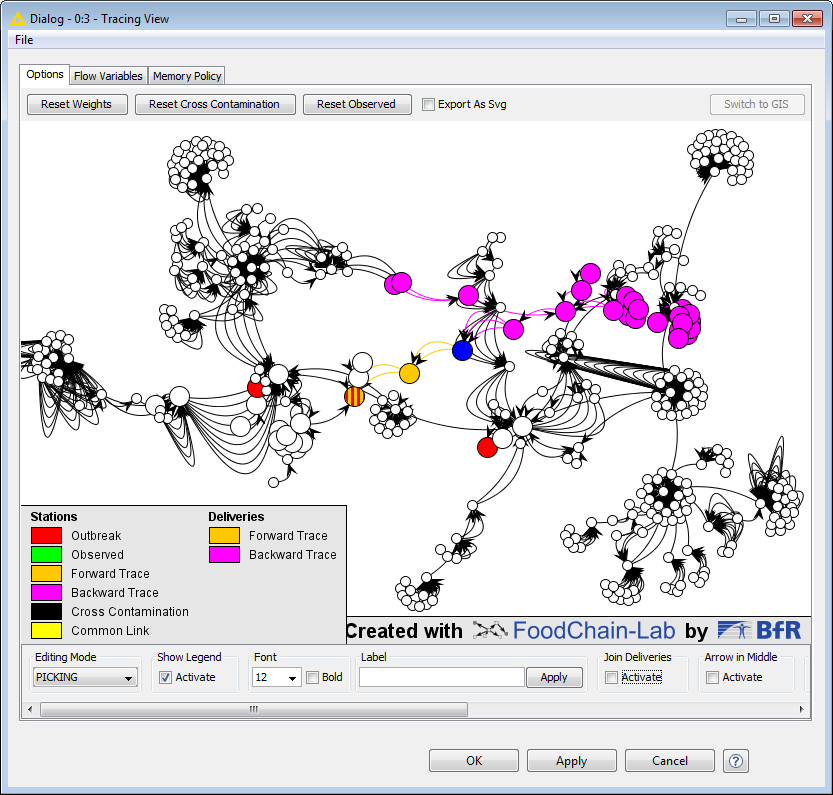
\includegraphics[height=0.6\textheight]{12.png}
	\end{center}
	\begin{itemize}
		\item Click at an empty area of the graph to unselect all stations.
		\item Now you can see, that the "Observed" station is green.
		\item Then activate "Join Deliveries" to simplify the graph. Deliveries with the same supplier and recipient are joined now.
	\end{itemize}
\end{frame}

\end{document}